\section{Zona de Estudio}

%--------------------------------------------------------

\begin{frame}{Zona de estudio}
	\begin{minipage}{0.5\textwidth}
		Datos Generales:
		\begin{itemize}
			\item Ubicación: 13°S, 75.1°W
			\item Superficie a evaluar: 23,000 Has (Aprox.)
			\item Rango de Elevaciones: 0-350 m
			\item Terreno homogéneo
			\item Clima desértico
			\item Tipo de cultivos: Alfalfa, Algodón, Espárrago, Mango, Maíz, Palta, Uva, Tomate.
		\end{itemize}
	\end{minipage} \hfill
	\begin{minipage}{0.45\textwidth}
		\begin{figure}
			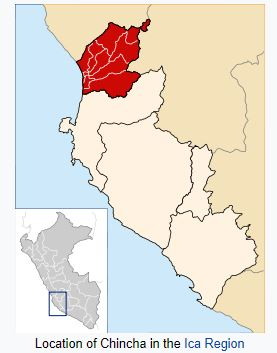
\includegraphics[scale=0.5]{imgs/chincha_ubic.JPG}
			\caption{Fuente: Wikipedia}
		\end{figure}
		
	\end{minipage}
\end{frame}

%---------------------------------------------------------

\begin{frame}{Zona de estudio}
	\begin{figure}[H]
		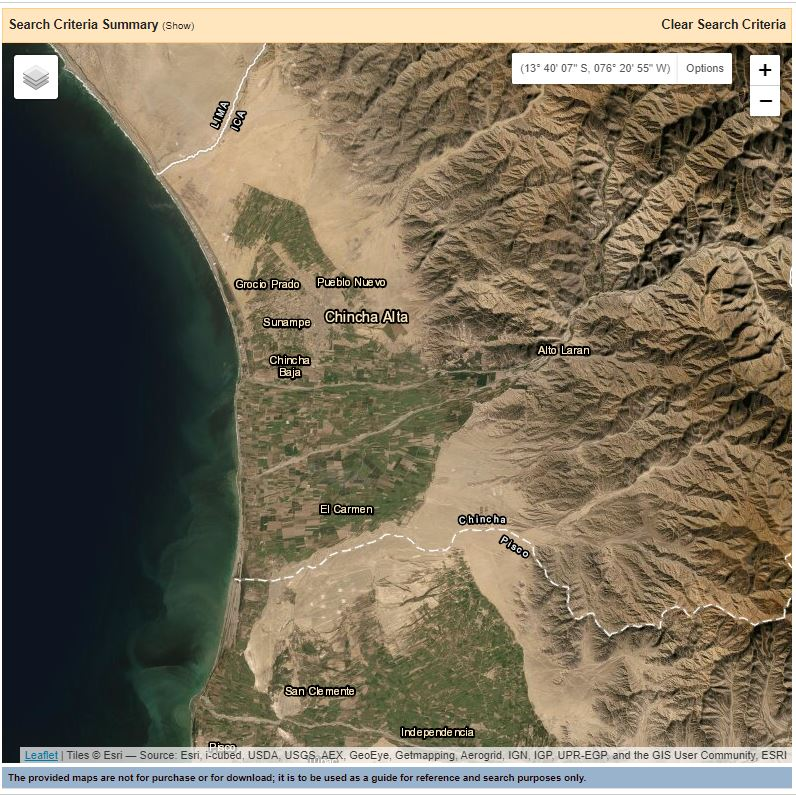
\includegraphics[width=0.75\textheight]{imgs/visualizacion_4.JPG}
		\caption{USGS Earthexplorer}
	\end{figure}
\end{frame}
